\saveSpace
\section{Validating encapsulated state}
\label{s:encapsulated}
\saveSpace
%Suppose we wanted to have a type and mutate it's state, but have such mutation's validated:


%It is very common for an object to be logically defined by the composition of sub-objects.
%The head object would then driving mutation of the sub-objects, and public methods
%of the sub-objects may be used in the validation. 
% However, the sub objects may come from a third party library, that is not annotated with contracts, and the %authors may change their behaviour in the future. Worst, they actual dynamic type may be dynamically loaded
%so that there is no way to predict their behaviour.
%That is, we are unable or unwilling to constrain sub-objects to
% cooperate into verification. We aim for verification to be correct independently of
% possibly buggy, possibly even malicious sub-objects.


Consider managing shipping items, where we keep an acceptable ship weight:
\saveSpace
%shipping list /UPS cost too much over 300
\begin{lstlisting}
class ShippingList {
  capsule Items items;
  read method Bool invariant() {
    return this.items.weight() <= 300;}
  ShippingList(capsule Items items) {
    this.items = items;
    if (!this.invariant()) {throw Error(...);}}//injected check
  mut method Void addItem(Item item) {
    this.items.add(item);
    if (!this.invariant()) {throw Error(...);}}}//injected check
\end{lstlisting}
\saveSpace
To handle this class we just inject calls to \Q@invariant@ at the end of the constructor and the \Q@addItem@ method.
This is safe since the \Q@items@ field is declared \Q@capsule@.
Relaxing our system to allows a \Q@mut@ modifier for
the \Q@items@ field and the corresponding constructor parameter 
makes the code broken:
the cargo we received in the constructor may be already compromised:
\saveSpace
\begin{lstlisting}
mut ShippingList l = new ShippingList(evilAlias);
// l is ok now, but we can break it
evilAlias.addItem(new HeavyItem()); // l is now invalid!
\end{lstlisting}
\saveSpace 
As you can see it would be possible for external code with no knowledge of the \Q@ShippingList@ to mutate its items.%
\footnote{
Conventional ownership solves these problems by requiring a deep clone of all the data the constructor takes as input, as well as all exposed data (possibly through getters).
In order to write correct library code in mainstream languages like Java/C++, defensive cloning~\cite{Bloch08} is needed.
%\REVComm{
For performance reasons, this is hardly done in practice and is a continuous source of bugs and unexpected behaviour~\cite{Bloch08}.}
%}{2}{citation to support this?}

Our restrictions on capsule mutators ensure that capsule fields are essentially an exclusive mutable reference.
Removing these restrictions would break our invariant protocol.
If we was to allow \Q@x.items@ to be seen as \Q@mut@ even if
\Q@x@ is not \Q@this@, then even if the \Q@ShippingList@ has full control at initialization time,
such control may be lost later:
\saveSpace
\begin{lstlisting}
mut ShippingList l = new ShippingList(new Items());
// l is ok now
mut Items evilAlias = l.items // here l loses control
// l is still ok
evilAlias.addItem(new HeavyItem()); // we invalidated l now
\end{lstlisting}
\saveSpace
If we allow for a \Q@mut@ return type this would be accepted:
\saveSpace
\begin{lstlisting}
mut method mut Items expose(C c) {return c.foo(this.items);}
\end{lstlisting}
\saveSpace
\noindent Depending on dynamic dispatch on \Q@c@, \Q@c.foo()@ may just be the identity function, thus
we would get in the same situation of the former example.
%Static analysis is usually unable/unwilling to track precise behaviour of dynamic dispatch.


%In addition to the above we put restrictions on any \Q@mut@ and \Q@capsule@ methods using a \Q@capsule@ field (we call such methods `capsule mutators'):
%\begin{itemize}
%\item only a single use of \Q@this@ is allowed (and is the one that uses the field),
%\item no \Q@mut@ or \Q@read@ parameters are allowed (apart from the implicit \Q@this@ parameter)
%\item and the return type cannot be \Q@mut@.
%\end{itemize}
%\noindent  Moreover, if the used capsule field is referenced in \validate, a \Q@this.validate()@ call is injected at the end of the method.


Allowing \Q@this@ to be used more then once can also cause problems:
\saveSpace
\begin{lstlisting}
mut method imm Void multiThis(C c) {
  read Foo f = c.foo(this);
  this.items.add(new HeavyItem());
  f.hi();} // Can `this' be observed here?
\end{lstlisting}
\saveSpace
\noindent If the former code was accepted, depending on dynamic dispatch on \Q@c@,
\Q@this@ may be reachable from \Q@f@, thus \Q@f.hi()@ may observe an invalid object.

In order to ensure that a second reference to \Q@this@ is not reachable through the parameters we only accept \Q@imm@ and \Q@capsule@ parameters.
If we were however to accept a \Q@read@ parameter, as in the example below,
we would be in the same situation as the former example, where \Q@f@ may contain
a reference to \Q@this@:
\saveSpace
\begin{lstlisting}
mut method imm Void addHeavy(read Foo f) {
  this.items.add(new HeavyItem())
  f.hi()} // Can 'this' be observed here?
...
mut ShippingList l = new ShippingList();
read Foo f = new Foo(l);
l.addHeavy(f); // We pass another reference to 'l' through f
\end{lstlisting}
\saveSpace

%, we would have the same problem with a \Q@read@ paramater. ... justify why we ned capsule
% The boat will sink if the weight of the cargo goes over 300. However, 
% \Q@Item@ and \Q@Items@ come from a third party library,  are not annotated with contracts and the authors may change their behaviour in the future. 
% All the code using \Q@Boat@  (client code) would like to  assume the boat has not sunk yet.
% In turn, that depends on the behaviour of \Q@Items.weight()@, thus the meaning of the \Q@Boat@ invariant is parametric on the everchanging meaning of  \Q@Items.weight()@.
% Can the code in the \Q@Boat@ class somehow enforce that for every possible well typed \Q@Item@ and \Q@Items@, client code will interact only with valid (non sunk)  boats?
% That is, we are unable or unwilling to constrain \Q@Item@ and \Q@Items@ to
% cooperate into making \Q@Boat@s unsinkable; 
% we aim to make so that \Q@Boat@s can be correct independently of
% possibly buggy, possibly even malicious \Q@Item@ and \Q@Items@ implementations.
% Indeed, thanks to the encapsulation, any kind of check in the language,
% as in `\Q@if(cargo.weight()>=300){..}@', would delegate the 
% behaviour to untrusted code in \Q@Items@.

% \textbf{without any knowledge about the behaviour of \Q@add()@ and \Q@weight()@}
% \footnote{A statically verified system with contracts on all methods may have this kind of knowledge.}
% there is no way we can discover the invariant violation without actually adding the objects and checking the 
% weight after the fact; thus in the general case violations can only be detected 
% when a broken object is already present in the system.
% Remember that to keep our approach lightweight,
% we do not rely on pre-post conditions; thus
% the behaviour of \Q@Items.weight()@ and \Q@Items.add(item)@ is uncertain.
% The names may suggest a specific behaviour, but there is no contract annotated on such methods.

% Note also that in the general case there is no way to fix a broken object,
%or to perform a deep clone and to test the operation on the clone first.


%REWRITE THIS BIT
%Here capsule fields 
%as input to our code-generation / \Q@validate()@-injection; that is, \Q@capsule T f@ is expanded by the language into:
%\begin{itemize}
%\item Induce a \Q@capsule@ parameter for the generated %constructor.
%\item Require to be updated with a \Q@capsule@ expression.
%\item Are accessed as a \Q@mut@ field.
%Access is \textbf{not} a destructive read.
% However methods accessing them are kept under
%strict control; either
%\begin{itemize}
%\item they have \Q@read this@: they act like a normal %getter, and can not propagate
%writing permission over the ROG of that field.
%Indeed, with \Q@read this@, any field access \Q@this.f@ will be typed \Q@read@ or \Q@imm@.
%\item they have \Q@mut this@, no parameter is \Q@mut@ or \Q@read@,
%the return type is not \Q@mut@ and \Q@this@ appear exactly one time in
%the method body: we call those methods \textbf{exposers}, and the invariant is going to be checked at the end of
%the exposers.
%\end{itemize}


%\end{itemize}
%Exposers are the key part of our solution.


% Those restrictions also enforce that while executing a capsule-mutator no object outside the ROG of \Q@this@ can be mutated, and thus capability objects cannot be usedI/O can not be performed: the capability objects are externally visible mutable objects and thus the type system will never place them into a \Q@capsule@.
%\subsection{The true expressibility of capsule modifiers}
%A capsule mutator method is a wrapper of a logical operation on a field, which is guaranteed to not see the \Q@this@ object.
%Thus, if \Q@this@ where to become broken during 
%the method's execution, we could not observe it until after. At first glance, it may seems that capsule %mutators allows for limited kinds of mutations.
%This is however not the case, consider the following
%general capsule mutator method that allows to apply any possible transformation over the content of a capsule %field:
%At first glance it mayseem from

\saveSpace
\section{Case studies}
\label{s:patterns}
\saveSpace

%interface Foo{ma mb}
%
%class Raw implements Foo{
%  no validate 
%}
%class ValidFoo1 implemens Foo{
%  private capsule Foo inner;
%  ma(){
%    this.inner.ma();
%  }
%  validate
%}
%
%
%class Raw {
%  mut method mut A stuff(read A a) {
%      if a.bar() {
%         x = ...
%      }
%      return new A(x)
%  }
%
%  read method imm Object stuffPre(read A a) {
%     return a.bar()
%  }
%  read method mut A stuffPost(imm Object o) {
%     return new A(x)
%  }
%  mut method imm Object stuffInner(imm Object) {
%      x = ...
%  }
%}
%class ValidFoo1 {
%	cpasule Raw r;
%  mut method mut A stuff(read A a) {
%     imm Object p = this.r.stuffPre(a);
%     imm Object res = this.transformR(r -> r.stuffInner(p));
%      return this.r.stuffPost(res)
%  }
%}
%
%
%
%class ValidFoo2 implemens Foo{
%  private capsule Foo inner;
%  validate
%}
\subsection{GUI}
Here we show that we are able to verify classes with circular mutable object graphs, that interact with the real world using I/O.
%Here we discuss how to use conventional OO programming patterns to take advantage of our system. Using those
%patterns allows to circumvent some of the apparent limitations of our system.
% At first glance it would seem that by only being able to validate immutable and encapsulated state one could not create validated classes with complicated, mutable interconnected object graphs.
%We show that this is not the case by encoding
%Our invariant is that everything in every movable container (and the top level component) should 
%-be inside the container 
%-not overlap with anyhing else inside
%Our containers represent boxes that completley contain other non-overlapping boxes.
Our case study involves a GUI with containers (\Q@SafeMovable@s) and \Q@Button@s;
the \Q@SafeMovable@ class has an invariant to ensure that its children are completely contained within it and do not overlap. The \Q@Button@s move their \Q@SafeMovable@ when pressed. We have a \Q@Widget@ interface which provides methods to get widget's size and position as well as children (a list of \Q@Widget@s). Both \Q@SafeMovable@s and \Q@Button@s implement \Q@Widget@. Crucially, since the children of \Q@SafeMovable@ is a list of \Q@Widget@s it can contain other \Q@SafeMovable@s, and all queries to their size and position are dynamically dispatched, such queries are also used in \Q@SafeMovable.invariant@.

% Gui where the graphic representation of the widgets are guaranteed to not overlap.
% \Q@SafeMovable@ is a \Q@Widget@ whose position can be dynamically changed.
% \Q@Widget@s can contains more widgets as children.
% The invariant of a \Q@SafeMovable sm@
% is that all \Q@Widget@s inside \Q@sm.children()@,
% do not overlap with each others, and are
% fully contained in the area of \Q@sm@.

% Crucially, one of the children may be another
% instance of \Q@SafeMovable@.

Here we show a simplified version\footnote{The full version, written in L42, which uses a different syntax, is available at \url{github.com/ElvisResearchGroup/L42/blob/master/Tests/src/widgetGui/libTests/SaveMovable.L42}}, where  \Q@SafeMovable@ has just one \Q@Button@, and certain sizes and positions are fixed. (Note: \Q@Widgets@ is a class representing a mutable list of \Q@mut@ \Q@Widget@s)
\begin{lstlisting}
class SafeMovable implements Widget{
  @Override read method Int left(){return this.box.l;}
  @Override read method Int top(){return this.box.t;}
  @Override read method Int width(){return 300;}
  @Override read method Int height(){return 300;}
  @Override read method read Widgets children(){
    return this.box.c;}
  @Override  mut method Void dispatch(Event e){
    for(Widget w:this.box.c){w.dispatch(e);}}
  capsule Box box;
  read method Bool invariant(){..}
  SafeMovable(capsule Widgets cs){this.box=mkBox(c);}
  static method capsule Box mkBox(capsule Widgets c){
    mut Box b=new Box(5,5,cs);
    b.c.add(new Button(0,0,10,10,new MoveAction(b));
    return b;}}//mut b is soundly promoted to capsule

class Box{ Int l; Int t; mut Widgets c;
  Box(Int l, Int t, mut Widgets c){..} }

class MoveAction implements Action{
  mut Box outer; MoveAction(mut Box outer){this.outer=outer;}
  mut method Void process(Event event){this.outer.l+=1;} }
..
void main(mut System system){
  system.newGui().display(new SafeMovable(..));}
\end{lstlisting}

As you can see, \Q@Box@es encapsulate the state of the \Q@SafeMovable@s that can change over time:
\Q@left@, \Q@top@, and \Q@children@. Also note how the ROG of \Q@Box@ is circular: since
the \Q@MoveAction@s inside \Q@Button@s need a reference to the containing \Q@Box@ in order to move it.
Even though the children of a \Q@SafeMovable@ are fully encapsulated we can still easily dispatch events to them by implementing \Q@Widget.dispatch@. Once a \Q@Button@ receives an \Q@Event@ with a matching ID it will then call its \Q@Action@'s \Q@process@ method. 

%Our main function uses a capability-object to display the top-level \Q@Widget@ and its \Q@children@, as well as dispatch events to it. 
Our example shows that the restrictions of TMs and OCs are flexible enough to encode interactive GUI programs, where widgets may circularly reference other widgets.
In order to perform this case study we had to first implement a simple GUI Library in L42. This library uses object capabilities to draw the widgets on screen, as well as fetch and dispatch the events. Importantly, neither our application, nor the underlying GUI library require back-doors into either our type-modifier or capability system to function, demonstrating the practical usability of our restrictions.


\textit{The Invariant:}
\Q@SafeMovable@ is the only class in our GUI that has an invariant, our system injects tests for it in two places: the end of its constructor and the end of its \Q@dispatch@ method (since it is a capsule-mutator). Their are no other checks inserted since we never do a field update on  \Q@SafeMovable@s. The code for the invariant is just a couple of simple nested loops:
\begin{lstlisting}
read method Bool invariant() {
  for (Widget w1 : this.box.c) {
    if(!this.inside(w1)) { return false; }
    for (Widget w2 : this.box.c) {
      if (w1 != w2 && SafeMovable.overlap(w1, w2)) {
        return false;}}}
  return true;}
\end{lstlisting}
Here \Q@SafeMovable.overlap@ is a static method that simply checks that the bounds of the widgets don't overlap. The call to \Q@this.inside(w1)@ similarly checks that the widget is not outside the bounds of \Q@this@; this instance method call is allowed as the function only uses \Q@this@ to access its fields.%its \Q@width@ and \Q@height@ fields.


% This code is a simplified version of our first case study. In the full code the \Q@SafeMovable@ constructors take \Q@left@, \Q@top@, \Q@width@ and \Q@height@ parameters and can either take a \Q@box@ directly or will generate one with $4$ \Q@Button@s}
% we we have $4$ buttons, each button moves in one of the $4$ cardinal directions.
\begin{wrapfigure}{l}{0.34\textwidth}
    \centering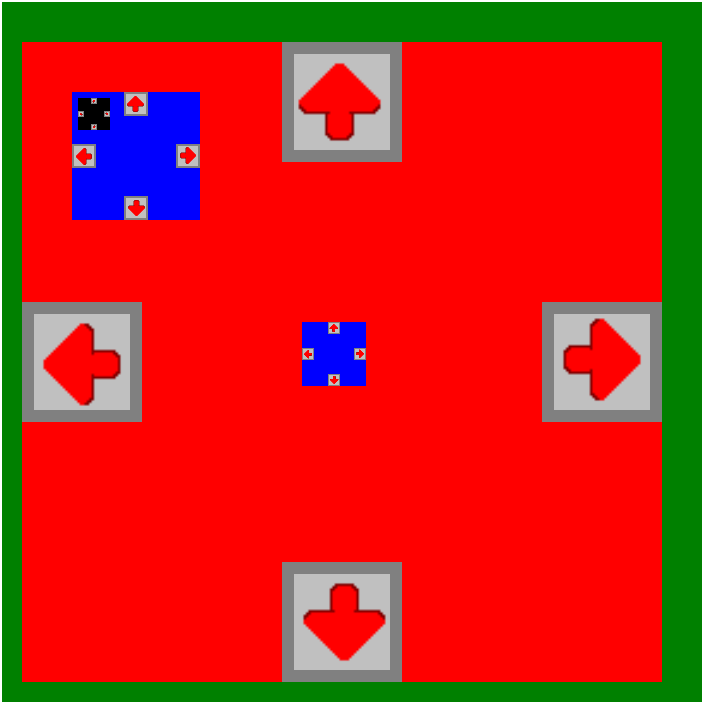
\includegraphics[width=0.34\textwidth]{GuiImg}\end{wrapfigure}
\noindent{\textit{Our Experiment:}} As shown in the figure, counting both \Q@SafeMovable@s and \Q@Button@s, our main method creates $21$ widgets: a top level (green) \Q@SafeMovable@ without buttons, containing $4$ (red, blue, and black) \Q@SafeMovable@s with
$4$ (gray) buttons each. When a button is pressed it moves the containing \Q@SafeMovable@ a small amount in the corresponding direction.
%Each container has 4 gray buttons one for each cardinal direction.
% In our set up
% the top level \Q@SafeMovable@
% contains a big red \Q@SafeMovable@
%  containing $2$ smaller blue \Q@SafeMovable@. One of those contains a tiny black \Q@SafeMovable@.
%Our invariant is that everything in every movable container (and the top level component) should 
%-be inside the container 
%-not overlap with anyhing else inside
%Our containers represent boxes that completley contain other non-overlapping boxes.
This set up is not overly involved, the maximum nesting level of \Q@Widget@s is $5$.
Our main method automatically presses each of the $16$ buttons once. In L42, using the approach of this paper, this resulted in $77$ calls to \Q@SafeMovable@s invariant.

\noindent{\textit{Comparison with visible state semantics:}}
As an experiment we set our implementation to generate invariant checks following the standard approach for visible state semantics (the one used by Eiffel and D), where the invariant is instead checked at the start and end of \emph{every} public method%
\footnote{
	%though 42 represents field accesses as method calls, for a fair comparison with conventional OO approach, we do not treat field accesses on \Q@SafeMovable@s within the \Q@SafeMovable@ class itself as public method calls
42 represents field accesses as method calls; 
in our experiment \Q@SafeMovable@ only access fields on \Q@this@ ...
for a fair comparison with other OO languages, we do not treat field accesses on \Q@SafeMovable@s within the \Q@SafeMovable@ class itself as public method calls
}
of \Q@SafeMovable@, including the simple getters implementing the \Q@Widget@ interface. When we ran our test case the invariant was instead called $52,734,053$ times (it took about $4$ days to run), in comparison to the $77$ we got when using our invariant protocol. The number of checks is exponential in the depth of the GUI: the invariant of a \Q@SafeMovable@ will call the \Q@width@, \Q@height@, \Q@left@, and \Q@top@ methods of its children, which may themselves be \Q@SafeMovable@s, and hence such calls will themselves invoke invariant checks. Note that like other systems in the literature, we do not perform invariant checks when calling instance methods on \Q@this@ within the invariant of \Q@SafeMovable@, had we done that we would have obviously gone into an infinite recursion.

% It can be surprising to see such extreme difference. We ran our example with less widgets, and our results suggest an exponential growth in the cost of the conventional approach. For example by removing 2 containers (and their 8 buttons) we get....
% We now explain how this exponential explosion happens:
% For the outer-most box to check its invariant, it needs to call methods \Q@left,top,height@ and \Q@with@ to all its contained widgets.
% If one of those widget has \Q@invariant@, when such public method is called,
% its \Q@invariant@ is checked (twice). This requires to call \Q@left,top,height@ and \Q@with@ to all its contained widgets, some of those may also have \Q@invariant@s.

% In literature there is attention to prevent method called from an invariant to call public methods on \Q@this@; it would cause the system to go in loop.
% However when calling methods on other objects is allowed, if those objects have invariant, this cause the aforementioned explosion. 

% Our example also shows that the restrictions of TM's and OC's are flexible enough to encode interactive GUI programs, where widgets may circularly reference other widgets.
% In order to perform this case study, we had to first implemented a simple Gui Library in L42. This library uses object capabilities to draw the widgets on screen, as well as fetch and dispatch the events.
% The gui library abstract away all the details of drawing and events; the user code need only to provide concrete classes implementing the \Q@Widget@ interface.

\noindent{\textit{Comparison with Spec\#}}
We encoded our Widget example also on Spec\#.
The result is the same of L42: the invariant is checked $77$ times, and in exactly the same locations of L42.
However, we found great difficulty to encode our example.
We used the Boogie static checker to verify all the aliasing-ownership properties needed to
ensure that the $77$ run-time invariant checks soundly enforce that the invariant holds when is expected.
This of course includes preventing the Gui to ever display two overlapping Widget. 

We believe this comparison is fair since we got both systems to essentially do the same thing:
they statically verify ownership/aliasing annotations,
they check the admissibility/valididty of a the invariant code and finally 
they perform sufficient runtime-checking of the invariant.
%\end{itemize}
To encode the GUI example in L42, we only needed to annotate using \Q@mut/read/capsule@, for a total of 
$19$ annotations (one token each, $74$ characters in total).
Spec\# required $40$ annotations, including methods
purity, ownership annotations on parameters, methods and field attributes as well as requires, ensures and modifies clauses, and finally also explicit ownership assignment statements.
Spec\# annotation can be involved, as for example \Q@requires Owner.Same(Owner.ElementProxy(children), children);@
To estimate the annotation burden we count the number of tokens (excluding \Q@.;,@ and parenthesis).
This gave us $113$ tokens, that is more then $5$ times the amount needed in L42.
The total annotation character count is $830$; $10$ times more then L42.
% 40   106+17=113 619+211
%main 11 annotations, 28 + 11 tokens, 118+65 characters
%safemovable 29 annotations, 78+6 tokens, 501+146 characters

%19   34   207+44
% auxLib // 14 annotations, 25 tokens, 155+44 characters
%guiLib// 5 annoations, 9 tokens, 52 characters




Moreover, in L42 we only use $3$ different kinds of annotations, while in Spec\# we use $15$ kinds of annotations. On the basis of those results we believe  that our system is easier to use for programmers that are not experts in software verification.

Our design, using an inner \Q@Box@ object is a common pattern in static verification: to encapsulate all the relevant mutating state into an encapsulated sub-object
that are never exposed to the users.
We also found natural to use the box pattern
also in Spec\# requires.
This dramatically simplifies the handling of the circular object graph, where the button event can refer back, in order to change the widget position.
Also the implementation of the minimal GUI library
(that our \Q@SaveMovable@ builds upon)
has a much lower annotation burden.

We encoded our Widget example also on Microsoft Code Contract; their system also ran the invariant checking $77$ times. Their system is easy to use, but it is unsound since it is built over an unsound/incomplete static verifier~\cite{?}.


\noindent\textit{The transform pattern:}
A capsule mutator method is a wrapper over a logical operation on a field, which is guaranteed to not see the \Q@this@ object.
Thus, if \Q@this@ is made invalid during 
the method's execution, we could not observe it until after the method completes.
At first glance, it may seem that capsule mutators allow only very limited kinds of mutation.
This is however not the case. 

Consider the following
simple pattern to allow flexible use of encapsulated content: define a \Q@transform@ function and a \Q@ItemTransformer@ interface like so:
\saveSpace
\begin{lstlisting}
interface Transformer<T>{method Void apply(mut T elem);}
interface Widget{..
  mut method Size setTop();//simple setters for immutable fields
  mut method Void transform(Transformer<List<Widget>> t);
  }//transformers for possibly encapsulated data
class SafeMovable{...
  mut method Void transform(Transformer<List<Widget>> t) {
   t.apply(this.box.c);
   if (!this.validate()) {throw Error(...);}}}//injected check
\end{lstlisting}
The \Q@.transform()@ method 
offers an expressive power similar to a
\Q@mut@ getter, but ensures that 
the field content cannot leak out.
For example:
\begin{lstlisting}[escapechar=\%]
// Lambda Expression that creates a new Transformer<...>
this.transform(l -> l.add(new MyWidget(..)))
\end{lstlisting}
%//`i' is captured by the closure.
%// `imm' and `capsule' varaibles can be captured.

%    %\Comment{}%this.items.add(i);
%    // Cant instead capture `this': it can't be typed %as `imm'
%    // since `ItemTransformer.transform()' is an %`imm' method
%  })
%}
%  // instead of:
  %\Comment{}%this.exposeItems().add(i)

Note that the code above does not access a capsule field but merely calls a method that does; thus
it is \emph{not} a capsule mutator method, so it is not constrained by the restrictions on them. Code like the above would also allow one to mutate multiple capsule fields in one method.
Our pattern cooperates with the language’s restrictions to ensure each mutation is completed as a separate operation, that is perceived by the rest of the system
as if it was atomic.%
%,  i.e. they can't see or update the other capsule fields.


\subsection{Family, a worst case scenario for L42}
%\noindent\textit{Family, a worst case scenario for L42}
For our second case study, we wished to make an example where the performance of L42 and the conventional approach was similar. We forged an example when a \Q@Family@ has a list of parents and a list of children;
all the children need to be younger then their parents and every \Q@Person@ need to have a non empty name and a positive age.  
We model the pass of time with a \Q@processDay@ method, and we simulate $3$ years of life (that is, $3\times365$ days) of a family of $4$.
The age of a \Q@Person@ grow when its birthday is processed.
Notably, \Q@processDay@ is a \Q@mut@ method that can potentially mutate any person in the system, thus
L42 have to run a lot of invariant checks. The object graph here is very shallow: the \Q@Family@ holds the \Q@Person@s and that is it.
However, even in this case we get about $9$ times less invariant calls: $19403$ with visible state semantic  and $2210$ in L42.
%Also the \Q@Family@ example uses the box pattern.

\subsection{Expressiveness}
%\noindent\textit{Expressiveness:}
Finally, in our this third case study we 
shown that even if we do not aim to expressiveness, but to simplicity, soundness and efficiency, we are still able to express a reasonable amount of cases.
We encoded in L42 all the examples present in papers~\cite{??}.
We can express all the examples except ....
Again, we quantify the annotation burden and we discover....

%\subsection{The transform pattern}


%\begin{lstlisting}[escapechar=\%]
%class List {
%  mut List prev;
%  mut List next;
%  Object elem;  
%  read method Bool ok() {
%    return this.next.prev==this && this.prev.next==this &&..;}
%  read method Int size(){
%    if(next==this){return 1;} return next.size()+1;}}
%\end{lstlisting}
%Clearly the \Q@mut@ fields of \Q@List@ cannot be marked as \Q@capsule@.
%However, only \Q@capsule@ and \Q@imm@
%fields can be accessed in \validate.
%Thus, \Q@.innerValidate()@ can not be the \validate{} method for \Q@List@.
%The solution is to use a `box' over our \Q@List@, and to validate our `box':
%
%\loseSpace\loseSpace\loseSpace
%\begin{lstlisting}[escapechar=\%]
%class ListBox { 
%  capsule List inner;
%  read method imm Bool invariant() {return this.inner.ok();}
%  read method Int size(){ return this.inner.size();}
%\end{lstlisting}
%\saveSpace
%Encoding this example in Spec\# would be much more verbose (see case study XX) and still require
%a \Q@ListBox@ object,
%while the visible state semantic of Eiffel or D would cause an large amount of \Q@invariant@ checks
%if the list had any recursive method; consider for example the \Q@size@ method:
%if there was an invariant with visible state semantic on \Q@List@, calling \Q@List.size()@ would require 
%calling \Q@List.invariant()@ before and after the method execution. If the list has more then one element, the recursive \Q@size@ call would also call the invariant twice.
%We would also want to create forwarding methods in \Q@ListBox@ for all public methods defined in \Q@List@. This approach allows the validation of many interesting and practically useful data-structures.
%However the limitations of capsule mutator methods mean that any \Q@mut@ methods in \Q@ListBox@ taking \Q@read@ or \Q@mut@ parameters, or returning \Q@mut@, cannot be trivially forwarded.
%% since they necessitate mutating a \Q@capsule@, instead complicated and involved forwarding would be needed, if it is even possible.
%Our example is about a list of immutable objects.
%To instead validate a list of \Q@mut@ objects we would need to use our box pattern not just around the list,
%but around a section of data encapsulating both the list and all the contained elements.
%This is because our simple \Q@capsule@ modifier requires the whole ROG to be encapsulated.
%Conceptually, it would be better for the list (of mutable objects) to be validated by its
%head, since the behaviour of the contained objects is transparent to the validation criteria. 
%Our limitation relates to full encapsulation and contrasts with flexible encapsulation as in 
%ownership~\cite{ClarkeEtAl98}. However, neither traditional flexible encapsulation/ownership, nor our language are capable of verifying that \Q@List.elem@ is not (indirectly) referenced within \Q@ListBox.validate()@.
%
